\chapter{Implementation}
In this chapter, we describe how we went about the implementation of the
debugger and reason about the design choices we made. Also, we describe which
parts of the virtual machine were modified or added to allow the implementation
of the debugger.

\section{T86 ISA Extensions}\label{section:parser}
In chapter~\ref{section:t86-vm}, we showed how to build a program for the T86
VM with the existing builder interface. To allow the usage of other programming
languages, we have created an ELF-like format for the T86 executables. The
format is a text one, making it easy to use. An example of a program in said
format is shown in figure~\ref{fig:t86-program}. It is very similar to the
assembly we have shown in previous sections. Thanks to this, students can
implement their compiler in any programming language they want and emit the T86
program in this format as a text file. An unfortunate side effect is that we
can no longer use the \texttt{DBG} instruction. However, the debugger we will
later present will be much more powerful than the \texttt{DBG} instruction.

As can be apparent from the example, we also use sections. The \texttt{.text}
section is the only mandatory one. It contains the instructions that will be
executed. Another one is the \texttt{.data} section. Here, either raw numbers
or strings can be written. The contents of this section are then loaded by the
VM and stored into the memory, beginning at memory cell 0 and upwards. There
are also debug sections, which we will present when discussing debugging
information.

\begin{figure}
    \begin{lstlisting}
.data
"Hello, World!\n"

.text
0   MOV [BP - 1], 0
1   JMP 8
2   MOV R0, [BP - 1]
3   MOV R1, [R0]
4   PUTCHAR R1
5   MOV R0, [BP - 1]
6   ADD R0, 1
7   MOV [BP - 1], R0
8   MOV R0, [BP - 1]
9   CMP R0, 13
10  JLE 2
11  HALT
    \end{lstlisting}
    \caption{Example of an T86 program which prints "Hello, World!".}
    \label{fig:t86-program}
\end{figure}
We will also add two new instructions. First is the \texttt{PUTNUM}
instruction, which prints the numerical value in the register and a newline.
This is intended as a very primitive debug instruction and to ease the
automated testing of the compiler. The only other way of output was to print a
char which was represented by the ASCII value. With this instruction, students
can bootstrap and test the basic implementation of their compiler more easily.

Another one is the \texttt{BKPT} instruction. This instruction is similar to
the \texttt{INT3} instruction from x86-64 or the \texttt{BKPT} instruction from
ARM. It is a software breakpoint. The virtual machine has no support for
interrupts, which are needed for debugging to work. This will be the focus of
the next section.

\section{T86 Debugging Support}
We could bake the debugger into the virtual machine itself, which would likely
be the simplest way to implement it. However, the goal of the debugger is not
only to ease the code generation part but to be a learning point so that
students might grasp how a real debugger works\footnote{The VM followed the
same philosophy.}. Because of this, we aim to simulate the real-world debuggers
as closely as possible. The compilers may also have more targets in the future,
not just the T86 VM. If we made the debugger part of the T86 VM, we could not
use it for a possible new virtual machine. In conclusion, the virtual machine
and the debugger will be two entirely different programs and, as such, two
completely different processes.

In the debugger implementation for Linux, the subject of section
\ref{section:linux-dbg}, we described how an operating system's kernel allows
the debugger's implementation via a specific API. There is no operating system
between the virtual machine and the program. Still, we will strive to make the
API similar to the ptrace API. The debugger and the VM will have to communicate
together somehow.

Both the VM and the debugger use an abstract class representing an interface
that provides two methods, \texttt{Send} and \texttt{Receive}. The
implementation of this interface then handles the concrete way of
communication. The debugger and VM do not care about it; they merely use these
two methods. There are currently two implementations of this interface. One is
using network communication through sockets. This way, the debugger may attach
to an existing process, even on an entirely different computer. It, however,
has a disadvantage. The messages sent are often short and we need to send a lot
of them. This proved too slow, even with few messages being sent. The second
implementation is via threads. The debugger runs the VM in another thread, and
they communicate via shared queues. This is much faster and allows the debugger
to run the process by himself, making it easier to use and behave like
real-world debuggers.

The format of the communication is a text one, merely because of the ease of
use as opposed to binary format. It is also clearer to see what is happening.
The commands that the debugging API of the virtual machine offers are
\begin{itemize}
    \item \texttt{PEEKREG x} - Return values of all normal registers.
    \item \texttt{POKEREG x y} - Set the value in register \texttt{x} to
        \texttt{y}.
    \item \texttt{PEEKFLOATREG} - Return values of all float registers.
    \item \texttt{POKEFLOATREG x y} - Set the value in float register
        \texttt{x} to \texttt{y}.
    \item \texttt{PEEKDEBUGREG} - Return value in all debug registers.
    \item \texttt{POKEDEBUGREG x y} - Set the value in debug register
        \texttt{x} to \texttt{y}.
    \item \texttt{PEEKDATA x cnt} - Return value in memory at addresses
        \texttt{x} to $\texttt{x} + \texttt{cnt} - 1$.
    \item \texttt{POKEDATA x y} - Writes a value \texttt{y} into a memory at
        address \texttt{x}.
    \item \texttt{PEEKTEXT x cnt} - Return instruction from \texttt{x} to $\texttt{x} + \texttt{cnt} - 1$.
    \item \texttt{POKETEXT x INS} - Rewrite the instruction at address
        \texttt{x} with the newly supplied instruction.
    \item \texttt{CONTINUE} - Continue the execution.
    \item \texttt{TERMINATE} - Stop the execution, terminating the virtual machine.
    \item \texttt{REASON} - Get the reason why the program stopped (breakpoint,
        singlestep, halt...).
    \item \texttt{SINGLESTEP} - Do native level single step.
    \item \texttt{TEXTSIZE} - Return the size of the program.
\end{itemize}

An example of how those commands can be used for communication between the
virtual machine and the debugger is shown in figure~\ref{fig:dbg-vm-seq}. The
interface is similar to basic ptrace commands. If the command should not return
anything, the VM sends back an \texttt{OK} message. We separate the memory and
instruction writing because T86 uses Harvard architecture, whereas Linux does
not separate text and data address spaces~\cite{ptrace}, so the two requests
were equivalent there. The API is made to be simple on purpose. Anything more
complex should be handled in the debugger itself.

\begin{figure}
    \centering
    \scalebox{0.8} {
    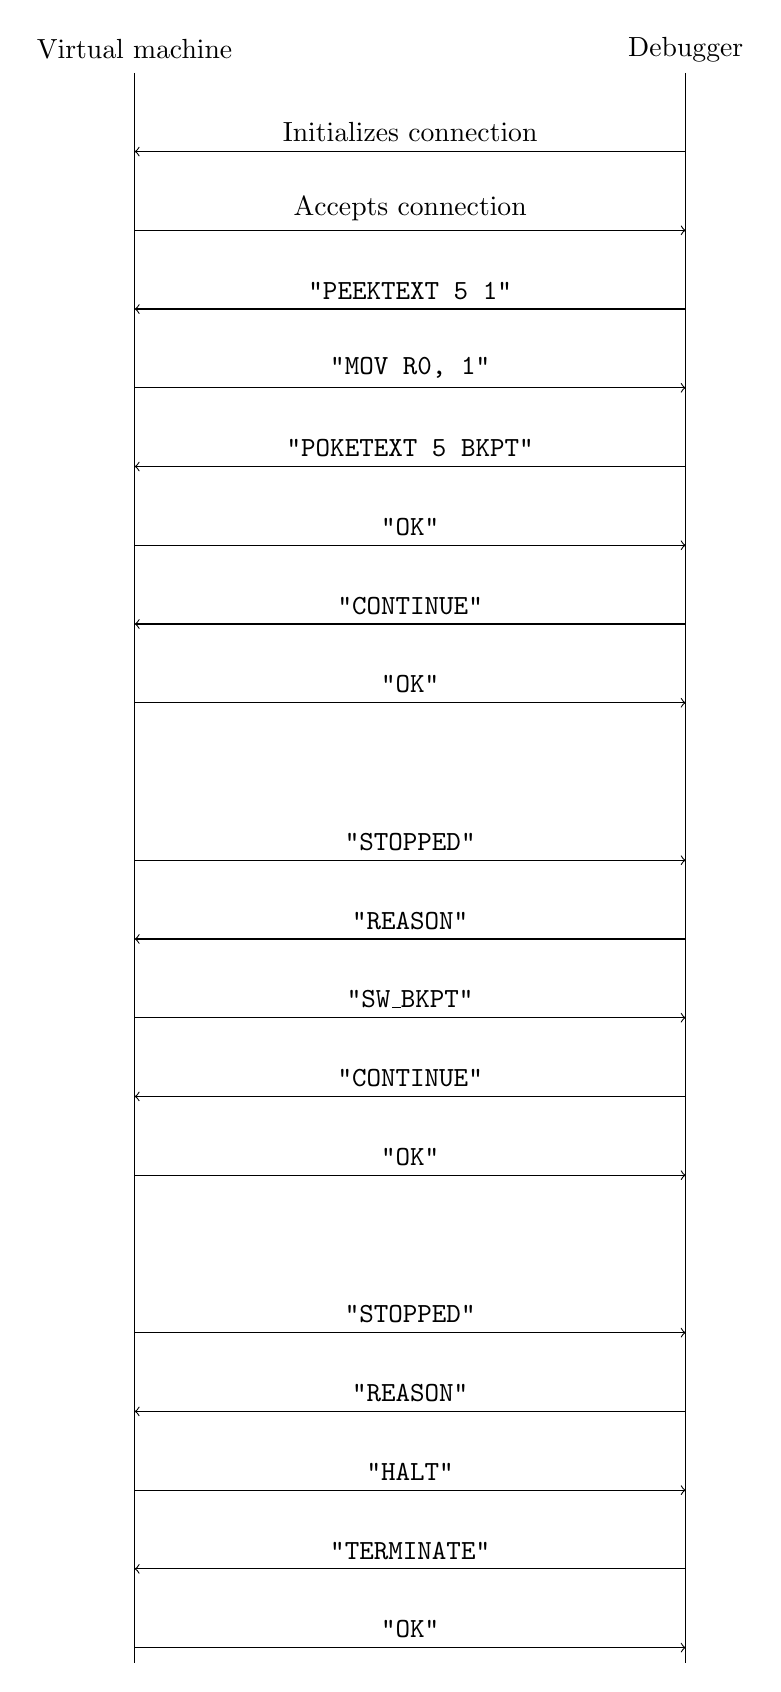
\begin{tikzpicture}
        \draw (0,0) -- (0,-20.2) (7,0) -- (7,-20.2);
        \node at (7,.3) {Debugger};
        \node at (0,.3) {Virtual machine};
        \draw[<-] (0,-1) -- node[midway,above] {Initializes connection} (7,-1);
        \draw[->] (0,-2) -- node[midway,above] {Accepts connection} (7,-2);
        \draw[<-] (0,-3) -- node[midway,above] {\texttt{"PEEKTEXT 5 1"}} (7,-3);
        \draw[->] (0,-4) -- node[midway,above] {\texttt{"MOV R0, 1"}} (7,-4);
        \draw[<-] (0,-5) -- node[midway,above] {\texttt{"POKETEXT 5 BKPT"}} (7,-5);
        \draw[->] (0,-6) -- node[midway,above] {\texttt{"OK"}} (7,-6);
        \draw[<-] (0,-7) -- node[midway,above] {\texttt{"CONTINUE"}} (7,-7);
        \draw[->] (0,-8) -- node[midway,above] {\texttt{"OK"}} (7,-8);
        \draw[->] (0,-10) -- node[midway,above] {\texttt{"STOPPED"}} (7,-10);
        \draw[<-] (0,-11) -- node[midway,above] {\texttt{"REASON"}} (7,-11);
        \draw[->] (0,-12) -- node[midway,above] {\texttt{"SW\_BKPT"}} (7,-12);
        \draw[<-] (0,-13) -- node[midway,above] {\texttt{"CONTINUE"}} (7,-13);
        \draw[->] (0,-14) -- node[midway,above] {\texttt{"OK"}} (7,-14);
        \draw[->] (0,-16) -- node[midway,above] {\texttt{"STOPPED"}} (7,-16);
        \draw[<-] (0,-17) -- node[midway,above] {\texttt{"REASON"}} (7,-17);
        \draw[->] (0,-18) -- node[midway,above] {\texttt{"HALT"}} (7,-18);
        \draw[<-] (0,-19) -- node[midway,above] {\texttt{"TERMINATE"}} (7,-19);
        \draw[->] (0,-20) -- node[midway,above] {\texttt{"OK"}} (7,-20);
    \end{tikzpicture}
    }
    \caption{A sequence diagram for the communication between the virtual
    machine and the debugger. If the label is enclosed in quotes, it is the
    actual text message that is being sent.} \label{fig:dbg-vm-seq}
\end{figure}

The \texttt{Cpu} class, which we have described in
section~\ref{section:t86-vm}, has no support for interrupts. The
\texttt{halted} method is kind of similar to interrupts but only allows for
signaling the \texttt{HALT} instruction execution. We need more than that.

We added another manager-like class called \textit{OS}. This class will take
care of running the program via the \texttt{Cpu} class. We also added an
\textit{interrupt} capability to the \texttt{Cpu}. To check if and which
interrupt happened, the \texttt{Cpu} now provides a function similar to the
\texttt{halted} function. The OS calls the \texttt{tick} method periodically,
and after every tick, it checks if a halt or interrupt occurred. If it did,
then it passes it to some handler. When an interrupt happens, unrolling must be
done to display proper values in registers and memory. This was described in
section \ref{section:superscalar-cpu}. The unrolling mechanism was fortunately
already implemented by the T86 VM author. It was used for the \texttt{DBG} and
\texttt{BRK} instructions, and we can use the same mechanisms for our addition
of interrupts.

The \texttt{BKPT} instruction we added is used for software breakpoints.
Executing this instruction causes an interrupt \texttt{3} to occur. It is also
possible to set a special flag that causes the \texttt{Cpu} to send the
interrupt \texttt{1} after every executed instruction. When an interrupt that
is caused by some debugging features happens, the \texttt{OS} calls a method in
the \texttt{Debug} class. This class is also a new addition and is responsible
for communication with the debugger. It uses the text protocol we mentioned
previously.

We also added debug registers. These are a special type of registers designed
for triggering breaks on memory access. There are a total of five debug
registers, with the first four containing the memory cell addresses. The fifth
register, called the control register, contains information about the debug
registers. The first four bits of this register indicate the state of each of
the first four registers. If the bit is set to one, then the register is
active. If a register is active and the program writes to a memory cell with
the same address as is stored in the register, an interrupt \texttt{2} is
generated. Furthermore, the control register's bits from 8 to 11 reveal which
register caused the interrupt. For instance, if bit 10 is set to 1, the third
register is responsible for the interrupt, and the address stored in that
register is the one that was written into.

\section{Native Debugger}
The implementation was done in the C++ language. It uses newer standards up to
the C++20 standard. The debugger is implemented as a library. We will call this
the backend of the debugger. A command line interface was also developed,
through which the users might interact with the debugger. This will be called
the frontend of the debugger.

The implemented debugger consists of two main parts. The first one aims to
support native (instruction) level debugging. This part works without
\textbf{any} debugging information whatsoever, ensuring it can be used by the
students immediately. The second part focuses on source-level debugging and is
described in section~\ref{section:source-debugger}.

The native debugger is split into two additional layers to make it more
modular. The first layer is called a \texttt{Process}. It is an interface
representing the debuggee process. The implementation of this interface is
responsible for dealing with the concrete architecture, the API of that
architecture, and the communication with the debuggee. One implementation is
provided for the T86 VM. For instance, it has a method called \texttt{ReadText}
and \texttt{WriteText}. The internals of these methods use the
\texttt{PEEKTEXT} and \texttt{POKETEXT} API we described. Outside of this
class, the communication API is never used. If, in the future, another virtual
machine is made, for whichever architecture, it is only needed to implement
this interface. The rest of the debugger can be used as-is.

Another layer is the \texttt{Native} class, which implements the complicated
logic behind a debugger, like setting a breakpoint, handling single-step, and
so forth. It is the primary bread and butter of the native part of the
debugger. Most algorithms are similar to the Linux debugger implementation
presented in section \ref{section:linux-dbg}. For illustration, in figure
\ref{t86dbg:breakpoint} we show a snippet of code used to create a breakpoint.
It first reads the text at the address where we want to set the breakpoint. The
breakpoint opcode then rewrites this text, and the backup of the text is
stored.

When we arrive at the breakpoint and want to continue further, we need to unset
the breakpoint, i.e., replace the breakpoint opcode in the T86 program with the
backup we saved, do a native-level single step, and write the breakpoint back.

Since breakpoints change the underlying code of the debuggee, we need to be
careful when presenting information to the user. If we printed the text that we
get from the debuggee, it might contain the \texttt{BKPT} instructions we set
earlier. We need to mix it with the backup code stored in breakpoints to show
the assembly of the program correctly.

The debugger also has a step-out and step-over functionality. The step-over
sets a breakpoint at the next instruction if the current instruction is a call
instruction. There is, however, one big problem with this approach, and that is
a recursive function. If a function is recursive, the recursive call might hit
this breakpoint. To prevent that, we look at the current value of the
\texttt{BP} register. The value of this register should be different in the
recursive calls because it is set in each function prologue. If the value of
the register is the same when the break happens, we consider the step-out
procedure complete. Otherwise, we will ignore the breakpoint hit and continue
the program execution.

With the step-out, we do single steps until we find a \texttt{RET} instruction.
We cannot use normal single steps but must use the step-over functionality.
Normal steps would cause us to enter a function and execute the \texttt{RET}
instruction there, which would mess with the algorithm.

The Native class uses a \texttt{DebugEvent} structure which indicates what
caused the VM to stop. It is implemented as a \texttt{variant} object
consisting of multiple structures, for instance, the \texttt{BreakpointHit} or
the \texttt{WatchpointTrigger} structure. It is a variant because the
watchpoint also needs to convey information about an address that caused the
break, as do breakpoints. It could also signal if the break was caused by
reading or writing to the memory cell, although for now, the T86 VM only
interrupts on writing.

\begin{figure}
    \begin{minted}{c++}
SoftwareBreakpoint CreateSoftwareBreakpoint(uint64_t address) {
    auto opcode = GetSoftwareBreakpointOpcode();
    // Read the text at the breakpoint address
    auto backup = process->ReadText(address, 1).at(0);
    // Rewrite it with the breakpoint opcode
    std::vector<std::string> data = {std::string(opcode)};
    process->WriteText(address, data);
    // Check that it was truly written
    auto new_opcode = process->ReadText(address, 1).at(0);
    if (new_opcode != opcode) {
        Error(...);
    }
    // Create a breakpoint object which keeps the text backup
    return SoftwareBreakpoint{backup, true};
}
    \end{minted}
    \caption{Debugger code in the \texttt{Native} class to enable a breakpoint.}
    \label{t86dbg:breakpoint}
\end{figure}

Here is a summarization of the features the native debugger offers:
\begin{itemize}
    \item Breakpoints - Can set, unset, enable and disable software breakpoints.
    \item Watchpoints - Can set and unset watchpoints on memory writes.
    \item Single stepping - Can do native level step into, which executes
        current instruction, out, which runs the program until it leaves
        current function and over, which treats function calls as a single
        instruction.
    \item Text manipulation - Can read and write into the debuggee text area,
        effectively allowing to overwrite the running code.
    \item Data manipulation - Can read and write into the program memory area.
    \item Register manipulation - Can manipulate with normal, float and debug registers.
\end{itemize}

\section{Debugging Source Code}\label{section:source-debugger}
With the solid foundation represented by the native part of the debugger, we
can extend it by providing some form of source-level debugging. For this part,
we need to remember that the debugger will only be used by students. As such,
we ought to have a somewhat simpler debugging information format than DWARF,
but we certainly can take inspiration from it.

As we previously mentioned, the executable with T86 code is separated into
sections. The \texttt{.text} and \texttt{.data} sections are for the VM. We
will introduce new sections where debugging information will be stored. All
those sections will have \verb|.debug_| prefix. The simplest new section is
\verb|.debug_source|, which should contain the original source code which was
compiled into this executable. This later allows us, with the combination of
other information, to display the source code lines.

The main philosophy of the source-level debugger is to allow an arbitrary
amount of debug information. For instance, the user can generate information
about one function only, and for that function, source debugging capabilities
will work, but not for any other. This means that users can generate debugging
information incrementally.

In the NI-GEN course, students are creating compilers from the TinyC language.
This is a small subset of the C language. It has simpler grammar and only
the following types: \texttt{int}, \texttt{double}, \texttt{char}, pointers,
structured types, and static arrays. We aim to support all of the TinyC
language in our source layer of the debugger.

The debugger is, however, not only limited to TinyC language. Any imperative
language that can be encoded with the following debugging information is
suitable to be debugged at the source level. We show an example of this in a
provided test case for the debugger where we debug the LLVM IR. It can be found
as an attachment to the thesis on path \texttt{impl/src/dbg-cli/tests/llvm.ir}.
We also provide documentation for developers who wish to generate this
debugging information in the thesis attachment on path
\texttt{impl/docs/source-info.md}.

The logic behind the source level debugging is mostly handled by the
\texttt{Source} class. It also stores all of the source level mapping, which we
are about to describe below. Some of the methods work closely with the
\texttt{Native} class to achieve functionality. That should not come as a
surprise, as we said, source-level debugging is built upon native-level
debugging.

\subsection{Line Information and Source Code}
The line information is encoded in a table, where every row is:
\texttt{<line>:<address>}. This is far simpler than the DWARF way, described in
section~\ref{section:line-number-information}. We do not care about being space
efficient, so we did a table instead of a virtual machine specification. We
also feel like this should be entry-level debugging information so that
students are not discouraged outright. It misses some information that DWARF
had, like columns. It still, however, proves quite sufficient for most cases.
The information should be stored in the \verb|.debug_line| section.

With this information, we are able to do source-level breakpoints. It is not
necessary to specify every line in the program. The debugger will refuse to put
a source-level breakpoint on some line if it does not have the necessary
information. If the source code is also provided, we can show the user on which
line is the debugged program currently paused. The source code should be under
the \verb|.debug_source| section, which must be the last section in the
executable.

\subsection{Debugging Information Format}
In the line information, we provided a straightforward format. However, we will
need a more sophisticated structure to describe some advanced constructs of the
source code. We will draw inspiration from the DWARF debugging information
entries. Take a look at figure~\ref{fig:t86dbg-die}, which shows an example of
such debugging information. It has a tree-like structure which, in some ways,
mimics the original program. The nodes of this tree are also called debugging
information entries (DIEs). Those entries can have other entries as their
children, and each entry has a tag that is part of its name (for example, the
\verb|compilation_unit| tag). They can also have attributes that describe their
properties. As can be seen, this is very similar to the DWARF debugging
information format. Unlike DWARF, it will be a text format. This allows us to
generate the format easily and to spot mistakes quickly. We do not want the
students to debug their generated debugging information.

For instance, the tag \verb|DIE_function| represents a function. As attributes,
it has a name, beginning address, and end address. With this additional
information, we can set a breakpoint on a function name. We can also display in
which function we are located when a break happens.

It also has one direct child, a \verb|DIE_scope|. The scope entry is mainly
used for keeping track of which variables are currently active because the T86
(or any other assembly language in general) has no notion of scopes. In the
scope entry in the example, only one variable called \texttt{d} exists. Thanks
to those entries, we can list currently active variables. We, however, often
need to examine the value of a variable. To achieve this, information about the
location and the variable type is needed. Global variables should be outside of
a function, as descendants of the \verb|compilation_unit| entry.

\begin{figure}
    \begin{lstlisting}
DIE_compilation_unit: {
DIE_function: {
    ATTR_name: main,
    ATTR_begin_addr: 0,
    ATTR_end_addr: 10,
    DIE_scope: {
        ATTR_begin_addr: 0
        ATTR_begin_addr: 10
        DIE_variable: {
            ATTR_name: d,
        },
    }
}
}
    \end{lstlisting}
    \caption{Debugging function information for the T86 debugger.}
    \label{fig:t86dbg-die}
\end{figure}

The type information is encoded as a standalone entry. Currently, four type
entries are present, one for primitive types (\texttt{int}, \texttt{double}, or
\texttt{char}), one for pointers, one for structured types (\texttt{struct} or
\texttt{class} in C++), and one for static arrays. Other types can be easily
added in the future. The types are saved as separate entries, and as such, we
need some way to link them together with the variables. We will use the
\verb|ATTR_id| attribute to achieve this. This attribute should be unique for
every entry, having a similar role to the \texttt{id} attribute of HTML
elements~\cite{html4}. The variables themselves have the \verb|ATTR_type|
attribute, which will have an id of the type as its value. An example of a
pointer type that points to an int type is in figure~\ref{fig:t86dbg-types}. If
we had a variable that is a pointer to an \texttt{int} type, it would need to
have the \verb|ATTR_type: 1| attribute because the id of a pointer type to
integer is one.

The primitive types need to have their size. For T86, this is the number of
memory cells it occupies, which will almost always be one since one memory cell
is 64 bits. It also has a name for its primitive type. Currently, three are
supported:
\begin{itemize}
    \item \texttt{int} - A signed integer.
    \item \texttt{float} - A floating point number.
    \item \texttt{char} - A number representing an ASCII character.
\end{itemize}

Additionally, we also support pointer types (including pointers to pointers),
static arrays, and structured types, which are a bit more complicated. They
need to have a list of members which are stored in the structure. For each
member, an offset from the beginning of the structure must also be specified.
It also must provide a size because the compiler might align it, and it may be
larger than the sum of the size of its members.

\begin{figure}
    \begin{lstlisting}
DIE_primitive_type: {
    ATTR_name: int,
    ATTR_id: 0,
    ATTR_size: 1,
},
DIE_pointer_type: {
    ATTR_type: 0,
    ATTR_id: 1,
    ATTR_size: 1
},
    \end{lstlisting}
    \caption{Debugging type information for the T86 debugger, showing an
    \texttt{int} primitive type and a pointer to \texttt{int} type.}
    \label{fig:t86dbg-types}
\end{figure}

With this information, we can show the type of a variable. Nevertheless, the most valuable thing is its value. Variables are either stored in memory, registered, or optimized out completely. We will follow DWARF's footsteps and provide a virtual machine specification.

The virtual machine is a stack-based one. After all instructions are executed,
the value at the top of the stack represents the resulting location. It can
either be a register or a memory offset. We offer several examples of programs
for the virtual machine:
\begin{itemize}
    \item \texttt{PUSH R0} - Pushes the register \texttt{R0}. No instructions
        remain, so the resulting location is the \texttt{R0} register.
    \item \texttt{PUSH BP; PUSH -2; ADD} - Pushes the \texttt{BP} register and
        the \texttt{-2} offset onto the stack. The \texttt{ADD} instruction
        pops two values from the stack and adds them together. If the value is
        a register, the value that is stored in that register is taken. The
        result from the addition is pushed back onto the stack.
    \item \verb|BASE_REG_OFFSET| - Does the exact same chain of operations as
        the previous example. Since the variables are often stored in memory at
        some offset from the base pointer, we provide this short hand.
\end{itemize}

There is also a dereference instruction, which dereferences a value in memory.
That can be useful for tracking the location of pointed variables. This virtual
machine is also easily extendable. With this kind of power, the location of
variables can almost be arbitrary and not only tied to a register or an offset
from the base register. This information is stored in a variable entry
attribute called \texttt{ATTR\_location}. If all this information is provided,
we know where the variable is stored and may look up its value. Together with
the type information, we might also properly interpret the value and report it
to the user.

\subsection{Source Expressions}
We could make a very straightforward implementation of getting variable value
by its name. It is only a matter of finding the variable entry with the correct
name and interpreting its location and type. However, we often need to inspect
some more complicated expressions. For example, we may want to display some
struct member or a value at which pointer points.

The debugger has a built-in interpreter for such expressions. It builds an AST
from the expression and interprets it using an AST
walk~\cite{crafting-interpreters}. The AST interpreter leverages the
\texttt{Native} class to fetch variable values. The interpreter supports almost
all C operators, including the assignment operator. It, however, has stricter
typing than C. An example of such an expression is \texttt{foo[2]->bar + 3}.
This is a very powerful feature, as it allows one to easily inspect or modify
various variables or expressions. If a user wishes to modify part of an array,
there is no need to use the raw memory or register setters. Instead, it is
possible to write \texttt{array[x] = y}.

The AST nodes are distinguished by types. They also need to store the location
of the expression if it is an expression that can appear on the left-hand side
of the assignment operator. Examples of expressions that must store the
location: \texttt{a}, \texttt{*(a + 1)}, \texttt{a[5]}, while the following
expressions do not have any locations because they cannot appear on the left
side of the assignment operator: \texttt{a + 1}, \texttt{5}, \texttt{array[0] *
y}.

\section{Frontend}
We provide two command-line interface programs. The first one is for the T86.
It runs the given T86 program on the virtual machine. The second application
leverages the debugger library to create a command line interface for the
debugger. It provides many commands, and its manual can be found in the thesis
attachment under path \texttt{impl/docs/debugging.md}. Additionally,
table~\ref{table:gdb-vs-dbg} shows examples of usage of the CLI compared to the
GDB debugger.

The main priority of the CLI is to make the debugger easy to use. It consists
of several commands, one of them is \texttt{breakpoint set 5}, which will set a
source-level breakpoint on the fifth line of the program. It is, however, not
necessary to write the whole command. Any prefix will do, like \texttt{b s 5}.
The CLI leverages the \textit{linenoise}~\cite{linenoise} library to make the
REPL satisfying to use.

The CLI also displays various information on program stop, like why the program
stopped, on which address or line, and prints the surrounding lines of assembly
or source. The CLI can also list breakpoints and display their locations in the
disassembly or the source code. Figure~\ref{fig:cli-hit} provides an example of
a breakpoint hit report. The debugger had all debugging information available
here. It can show the line in the source code where the breakpoint happened,
name the offending function, and variables in scope.

When variable values are printed, the format tries to accommodate their type.
For example, variables that are arrays or pointers to the \texttt{char} type
print the value of the variable as a string literal.

\begin{figure}
    \begin{lstlisting}
Process stopped, reason: Software breakpoint hit at line 11
function main at 7-18; active variables: a, b
      9:    int b = 6;
     10:    swap(&a, &b);
@->  11:    print(a);
     12:    print(b);
     13:}
    \end{lstlisting}
    \caption{Example of the debugger CLI reporting a breakpoint hit.}
    \label{fig:cli-hit}
\end{figure}
